
\chapter*{Abstract}
	\begin{abstract}
	Les images gigapixel ont un grand nombre d'applications, de l'art à la médecine en passant par la cartographie. Et plus 
	récemment, les jeux vidéos. Les techniques photographiques permettant de les générer ne manquent pas, l'espace stockage 
	et la bande passante non plus. Cependant les possibilités d'édition et de retouche numérique étaient jusqu'à présent 
	très limitées, aucun framework d'édition d'image ne se révélant satisfaisant. Une ébauche d'un nouveau concept de framework,
	conçu et réalisé par l'auteur, promettait des performances quasi indépendantes de la taille de l'image éditée, permettant ainsi 
	l'édition interactive d'images gigapixel

	Afin de vérifier ces promesses, l'implémentation du framework fut partiellement complétée, afin de se concentrer sur un problème restreint;
	la peinture d'images gigapixel. Cela révéla des problèmes de qualité et de performances,
	qui furent pour la plupart résolus de manière satisfaisante. Un logiciel de peinture utilisant ce framework fut ensuite 
	complété puis testé par 3 professionnels de l'art numérique afin d'évaluer la performance du framework et de son implémentation. 

	Les tests se sont conclus par la satisfaction des testeurs et la réalisation de plusieurs peintures gigapixel. 
	
	De nombreuses fonctionnalités du framework restent cependant à implé\-menter et à tester, de même que de nombreuses pistes
	d'amélioration des performances ont été ouvertes et restent à explorer.
	\end{abstract}
	

\chapter*{Préface}
	Ce rapport présente le résultat de mon mémoire réalisé au département de recherche en infographie de la \emph{Katholieke Universiteit Leuven}.
	Ce mémoire est également la conclusion de mon master d'ingénieur en informatique à L'\emph{Université Catholique de Louvain}.

	J'aimerais remercier les personnes suivantes: Philip Dutré de la KUL, et Marc Lobelle de l'UCL pour avoir été mes promoteurs,
	et Benedict J. Brown pour les avoir assisté dans cette tâche. J'aimerais également remercier les mémorants du département de recherche en infographie
	de la KUL pour leurs discussions et commentaire à propos de ce mémoire. 

	Enfin j'aimerais remercier Brice Vandemoortele, Jean-François Brogniet et Jean-Philippe Servais pour avoir participé aux tests utilisateur.

\chapter{Introduction}
	Les images gigapixel sont des images bitmap constituées de plus d'un milliard de pixel. Ces images apparaissent dans plusieurs domaines: la cartographie,
	avec les photographies satellites; la médecine, avec les images issues des microscopes; l'histoire et la préservation de l'art, avec des scans haute 
	résolutions de tableaux et fresques de grande taille; L'art numérique et également les jeux-vidéo qui utilisent de telles images pour la création
	de larges environnements. 

	Les algorithmes de compression et le faible coût de l'espace disque permettent de stocker sans encombre de telles images. Il existe également des logiciels
	de visualisation efficace. Cependant, lorsqu'il s'agit de les éditer, les logiciels existant ne proposent qu'une sélection très réduite des fonctionnalités
	proposées habituellement pour l'édition d'image mégapixel.  

	L'édition de telles images requiert une approche et des algorithmes différents. C'est ce que propose le framework nommé \emph{Himalaya}, conçu et
	partiellement implémenté au préalable par l'auteur de ce mémoire.  \emph{Himalaya} est un framework conçu pour pouvoir proposer la plupart des
	fonctionnalités des frameworks existants, avec des performances quasi indépendantes de la taille de l'image à éditer. 

	Cependant il y a un pas entre la conception et la réalisation, pas que nous avons partiellement franchi avec ce mémoire. En effet, l'implémentation
	complète du framework est une tâche d'une trop grande ampleur pour être envisagée ici. Nous avons donc fait le choix de se concentrer sur un
	sous-problème difficile, qui est de permettre de peindre de manière interactive une image gigapixel, fonctionnalité qui n'est proposée par aucun
	framework existant.

	Avant d'examiner en détail le framework \emph{Himalaya} il est important de se demander ce qu'est un framework d'édition d'image, quelles sont les
	fonctionnalités utiles et nécessaires de ceux-ci. Enfin il faudra regarder de quelle manière les frameworks existants proposent ces fonctionnalités,
	afin de comprendre les enjeux de conception. C'est ce que nous allons faire au prochain chapitre. 
	
	
\chapter[Présentation des frameworks d'édition d'images][Frameworks d'édition d'images]{Présentation des frameworks d'édition d'images}
	

	Un framework est une librairie présentant une interface logicielle permettant à un utilisateur d'éditer des images. 
	
	\index{Framework d'édition d'images}
	Le terme utilisateur sera employé pour désigner en toute généralité des choses assez différentes. Ainsi il désignera parfois 
	l'artiste qui utilise le logiciel d'édition, le programmeur qui utilise le framework pour
	concevoir un logiciel, mais aussi un autre programme qui ferait appel à celui ci.  

	Nous allons tout d'abord examiner quels sont les éléments qui constituent un tel framework, ensuite quels sont
	les fonctionnalités qu'ils doivent présenter à l'utilisateur. 

	Ensuite un survol des différents frameworks permettra des principes généraux de la conception d'un framework d'édition d'image.
	
	Pour réaliser cette présentation je me suis basé sur une lecture du code source des différents frameworks open-source, afin d'évaluer
	les structures de données et les algorithmes utilisés. J'ai également étudié les fonctionnalités et performances des logiciels fermés,
	qui bien que gardant secret leur fonctionnement, proposent généralement de meilleures performances et un plus large panel de fonctionnalités.
	
	Enfin, une étude des spécifications des principaux formats de fichiers standards permet de se rendre compte des fonctionnalités qui sont 
	attendues dans les frameworks. 

	Après chaque description de chaque framework on trouvera la liste des formats et logiciels ainsi examinés.

	\section{Architecture d'un framework d'édition d'image}
		Un framework d'édition d'images est composé de trois éléments principaux : 
		\begin{description}
			\item[Schéma de représentation de l'image]: Ce schéma est constitué de structures de données qui 
			décrivent l'image et les modifications qui lui sont apportées. 
			\item[Algorithme de rasterisation]: Cet algorithme permet d'obtenir une version matricielle de l'image,
			ou d'une partie de celle-ci. Une telle opération est indispensable car seule la forme matricielle de l'image
			peut être affichée à l'écran.
			\item[Algorithmes d'édition du schéma]: Ces algorithmes vont modifier la représen\-tation de l'image afin 
			d'implémenter les différentes fonctionnalités du framework.
		\end{description}

	\section{Fonctionnalités d'un framework d'édition d'image}
		\subsection{Opérations de dessin}
			L'opération de base d'un framework d'édition d'image est bien évidemment de permettre de 
			modifier une image. On distingue plusieurs manières de le faire qui seront traitées différemment
			selon les implémentations.
			\subsubsection{Dessin de primitives}
				Par dessin de primitive on entend l'ajout sur l'image de primitives géométriques, comme
				des polygones, des lignes, des points, des ellipses, du texte, etc. Ces primitives ont généralement un 
				effet local sur l'image, c'est à dire qu'elles ne la modifient pas dans son intégralité. 

				On différencie deux approches du dessin de primitive: L'approche dite vectorielle ou l'on utilise un 
				nombre réduit de primitives complexes (texte, courbes de bézier,...), et l'approche bitmap ou l'on utilise
				un très grand nombre de primitives très simples(ellipses, petits bitmaps, ...) qui prennent peu ou pas
				de ressources. 

				L'approche vectorielle permet de décrire facilement et efficacement des images très structurées, telles
				que des document textes, des graphes, des schémas techniques, ou des dessins schématisés. 

				Les techniques de graphe de scène (voir la section \emph{Frameworks Vectoriels}) s'adaptent très bien
				à cette approche et permet de structurer ces images de manière spatiale et sémantique.

				Le nombre quasiment illimité de primitives que permet la seconde approche rend possible la description
				d'images totalement déstructurées telles que les peintures.

				Puisque nous voulons développer un framework de peinture d'images gigapixel, c'est vers cette
				seconde approche que nous devons nous tourner. 

				\index{Primitives, dessin de}
				\begin{figure}[h]
					\centering
					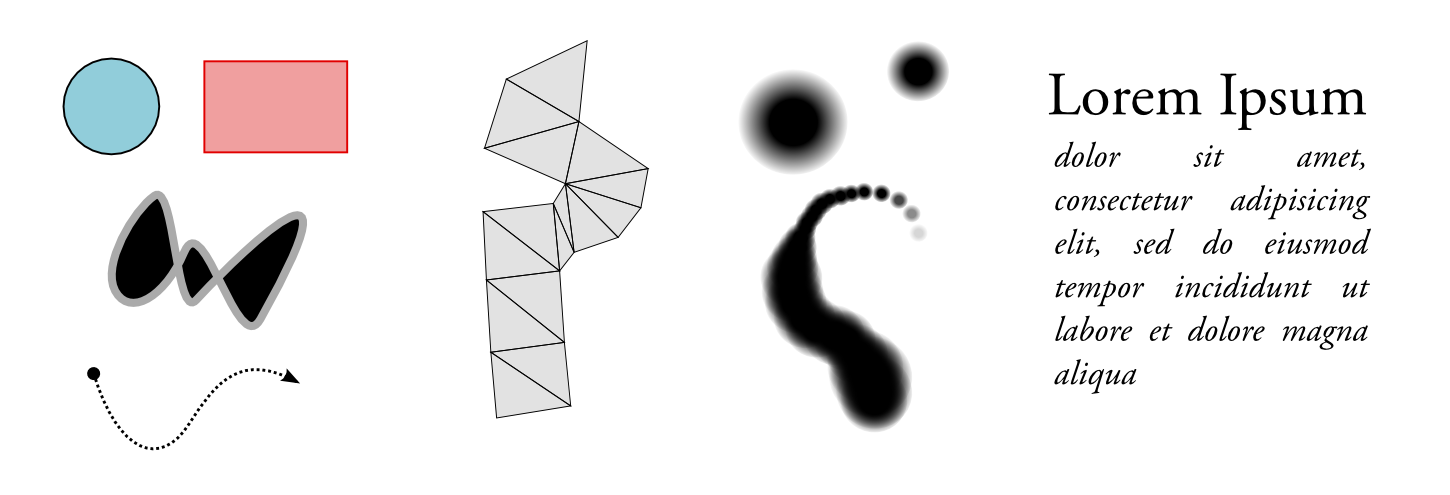
\includegraphics[width=\textwidth]{images/primitives}
					\caption{Exemples de dessins de primitives}
					\label{fig:primitives}
				\end{figure}
			\subsubsection{Filtres}
				\index{Filtres}
				Un filtre est une opération qui modifie l'aspect de l'entièreté d'une image. Le temps de calcul d'un filtre varie
				énormément d'un filtre à l'autre. Les plus simples prennent quelques microsecondes et peuvent aisément être exécutés
				en temps réel. D'autres prennent plusieurs dizaines de minutes\footnote{Un exemple récent est le \emph{Content Aware Filling}, \cite{contentaware}}. Certains frameworks ne sauront intégrer que les filtres
				les plus rapides. 

				Les filtres peuvent être également partagés en deux catégories,\index{Filtres!colorimétriques} les filtres colorimétriques qui transforment
				la couleur d'un pixel sans se soucier de la couleur des pixels voisins, \index{Filtres!spatiaux} et les filtres spatiaux nécessitant 
				eux d'en connaître plusieurs. 
				\begin{figure}[h]
					\centering
					\subfloat[Image originale]{ \label{fig:lenna_a} 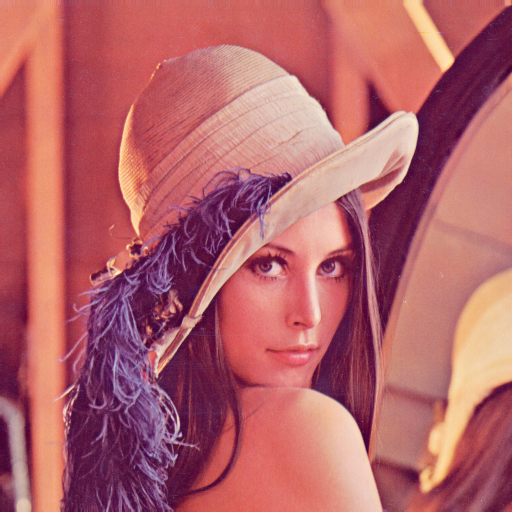
\includegraphics[width=0.3\textwidth]{images/Lenna} }
					\subfloat[Filtre colorimétrique]{ \label{fig:lenna_b} 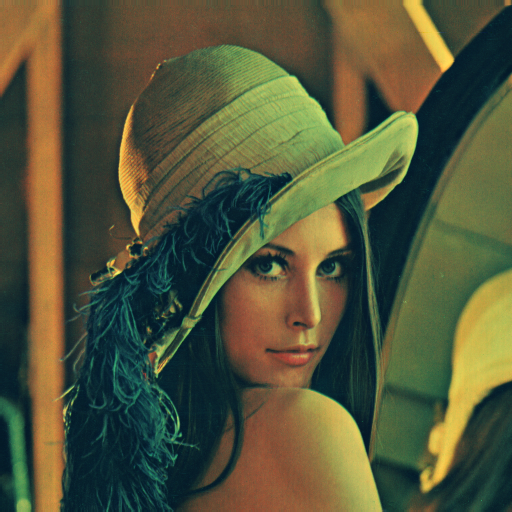
\includegraphics[width=0.3\textwidth]{images/Lenna-green} }
					\subfloat[Filtre spatial \emph{Sobel}]{ \label{fig:lenna_c} 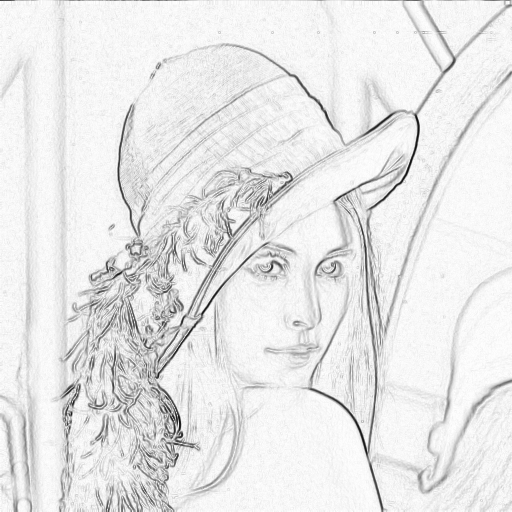
\includegraphics[width=0.3\textwidth]{images/Lenna-sobel} }
					\caption{Exemples de filtres}
					\label{fig:filtres}
				\end{figure}
			\subsubsection{Transformations géométriques}
				Les transformations géométriques modifient la forme d'un objet constituant l'image; rotation, translation, 
				redimensionnement et perspective sont les applications les plus courantes. 
				
				Il y a deux approches pour implémenter les transformations
				géométriques: l'approche vectorielle consiste à modifier la description de l'image avant la rasterisation. L'approche
				bitmap consiste à modifier les pixels après leur rasterisation. Cette deuxième approche, nettement plus lente, permet
				cependant d'implémenter des transformations non linéaires, telle que les transformées polaires, la correction de distorsion de 
				lentille, ou les déformations fluides. 
				
			\subsubsection{Fusion et modes de fusion}
				La fusion consiste à fusionner deux images en une. On utilise pour cela une fonction nommée \emph{mode de fusion}.
				Elle à la forme $f(p_A ,p_B ,\alpha)$, où $p_A$, $p_B$ sont deux pixels des images $A$,$B$ que l'on veut fusionner. 
				$\alpha$ représente un ou plusieurs paramètres additionnels qui peuvent	modifier l'effet de la fonction.

				Le \emph{mode de fusion} la plus courante est celui de mélange par opacité: $f(p_A, p_B, \alpha) = \alpha * p_A + (1-\alpha) * p_B$,  $\alpha \in [0,1]$ 
				représentant l'opacité de $B$, mais il en existe bien d'autres.

				On peut utiliser cette fonction pour fusionner deux images en une nouvelle : $ C = f(A,B,\alpha)$, ou pour intégrer une image dans
				une autre $A = f(A,B,\alpha)$

				Puisque chaque dessin de primitive consiste en la fusion de celle ci sur l'image de fond, la fusion est une opération centrale
				dans tout framework. Cependant beaucoup d'entre eux se limitent au seul mode de mélange par opacité.

				\begin{figure}[h]
					\centering
					\subfloat[Image A]{ \label{fig:A} 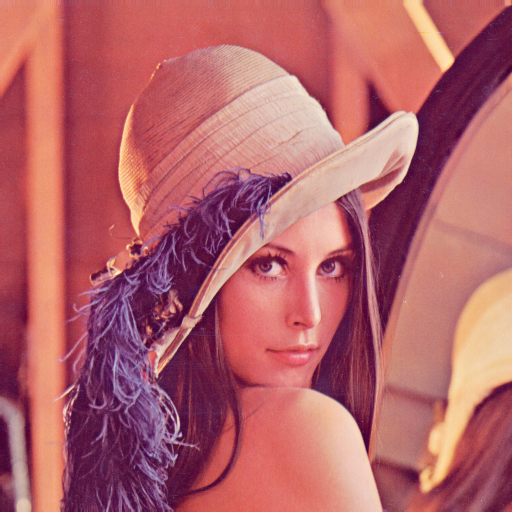
\includegraphics[width=0.25\textwidth]{images/Lenna} }
					\subfloat[Image B]{ \label{fig:B} 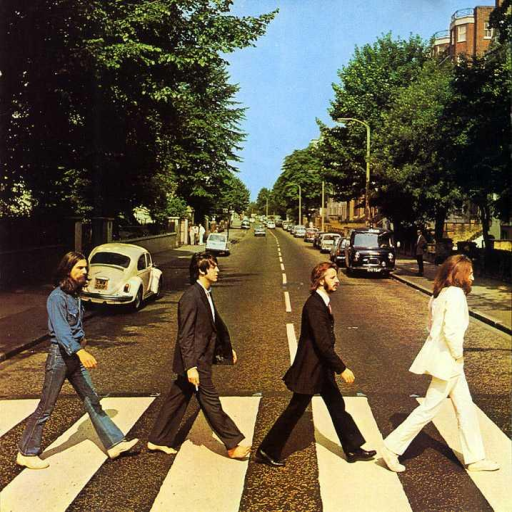
\includegraphics[width=0.25\textwidth]{images/abbey-road} }
					\subfloat[Blending de B sur A, par \emph{fusion de grain} ]{ \label{fig:ABfusion} 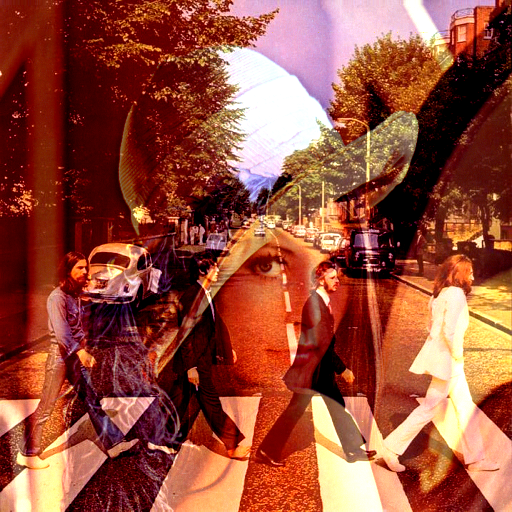
\includegraphics [width=0.25\textwidth]{images/abbey-road-lenna-fusion} }
					\subfloat[Blending de B sur A, par \emph{soustraction} ]{ \label{fig:ABsoustraction} 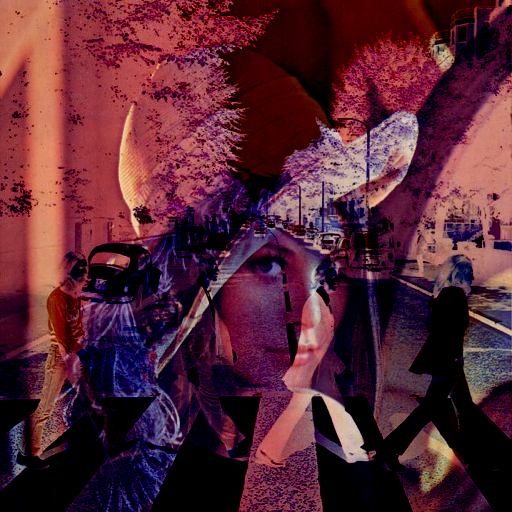
\includegraphics [width=0.25\textwidth]{images/abbey-road-lenna-substract} }
					\caption{Exemples de blending}
					\label{fig:blending}
				\end{figure}

		\subsection{Modèles colorimétriques}
			La rasterisation d'une image permet de définir la couleur de chaque pixel. Or il existe de nombreuses manières de définir une même couleur.
			La manière la plus populaire est de définir la couleur comme un vecteur dans un espace colorimétrique. Chaque espace ayant sa propre utilité:
			\begin{description}
				\item[Le RGB] est l'espace utilisé par les écrans et projecteurs, ainsi que les capteur photographiques. Toute couleur doit donc être
				convertie en RGB avant d'être affichée. Il existe plusieurs espaces RGB définis par des couleurs primaires Rouges, Vertes et Bleues différentes.
				Le plus utilisé est le sRGB, qui est le standard d'affichage des écrans\cite{reviewrgb}.
				\item[Le Yuv] est l'espace utilisé par les vidéos et par certains formats de fichier comme le JPEG.
				L'espace Yuv permet en effet une meilleure compression des données.
				\item[Le CIELab] est l'espace utilisé en retouche photo, il permet de manipuler les couleurs de manière conforme à la perception humaine.
				\item[Le HSL] est un espace qui permet de décrire les couleurs en composantes de teintes, de saturation et de luminosité, notions
				facilement compréhensibles et manipulables. Cet espace est utilisé pour certains filtres et pour l'édition des couleurs.
				\item[Le CMYK] est l'espace utilisé par les imprimantes jet d'encre, chaque imprimante ayant ses propres couleurs primaires. 
				Toute image doit donc être convertie dans le CMYK correspondant à l'imprimante avant d'être imprimée.
			\end{description}
			Il existe encore bien d'autres espaces colorimétriques spécifiques à des applications industrielles particulières. 

			Pour compliquer le tout, les espaces colorimétriques ne se superposent géné\-ralement pas. Ainsi des couleurs qui peuvent s'exprimer dans l'un n'existent pas
			dans l'autre. Un framework dédié à l'impression doit ainsi prendre garde de n'afficher en RGB que des couleurs disponibles dans le CMYK de l'imprimante.

			Une autre manière de décrire les couleurs est d'utiliser un nuancier contenant une liste de couleurs standardisées. Ce système est utilisé dans les images destinées à l'impression
			afin d'identifier des encres dont l'apparence ne peut être réduite à une simple couleur, comme les encres mattes, brillantes, métallisées,
			fluorescentes, etc. Dans ce cas chaque pixel possède une certaine quantité de chacune des  couleurs utilisées pour décrire l'image.

			\subsubsection{Quantisation}
			Les composantes d'un pixel peuvent aussi être quantifiées à différents degrés: 1bit pour les systèmes halftone; 8bit pour l'affichage 
			à l'écran,  les textures de jeux-vidéo; 32 bit flottant pour avoir des valeurs de couleurs dépassant les capacité d'affichage
			d'un écran, ce qui est particulièrement intéressant pour l'édition non destructive d'image utilisée en photographie et en 
			effets spéciaux. La précision apportée par une telle profondeur est également indispensable pour le cinéma numérique.

			\subsubsection{Extensions de modèles colorimétriques}

			Enfin, il arrive qu'un pixel ne décrive plus une couleur mais une information quelconque de la partie de l'objet qu'il représente.
			On rencontre ainsi la distance du pixel à l'observateur, la normale de la surface, un identifiant unique de l'objet, la vitesse de
			déplacement de l'objet, etc. Ces informations sont généralement fournies en plus des informations colorimétriques habituelles.

			Ce type d'information est typiquement fourni par la caméra ou généré par le moteur de rendu afin de faciliter l'intégration d'effets
			spéciaux à l'image. Les types d'informations utilisés apparaissent et disparaissent avec les technologies, nécessitant une grande 
			flexibilité dans leur gestion. Les \emph{Éditeurs Nodaux} sont particulièrement adaptés à la gestion de ce type d'informations.
			
			\begin{figure}[h]
				\centering
				\subfloat[Couleurs vraies]{ \label{fig:render} 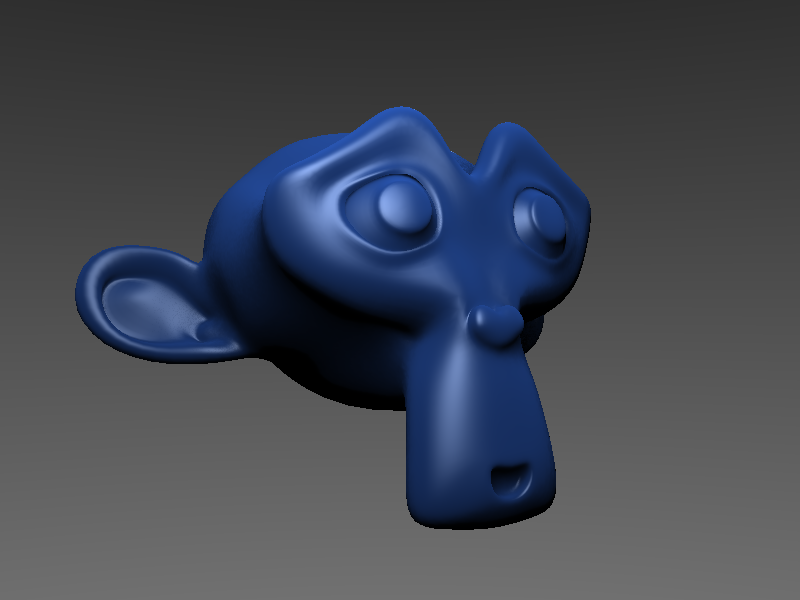
\includegraphics[width=0.25\textwidth]{images/render} }
				\subfloat[Format HSL en fausses couleurs]{ \label{fig:render-hsv} 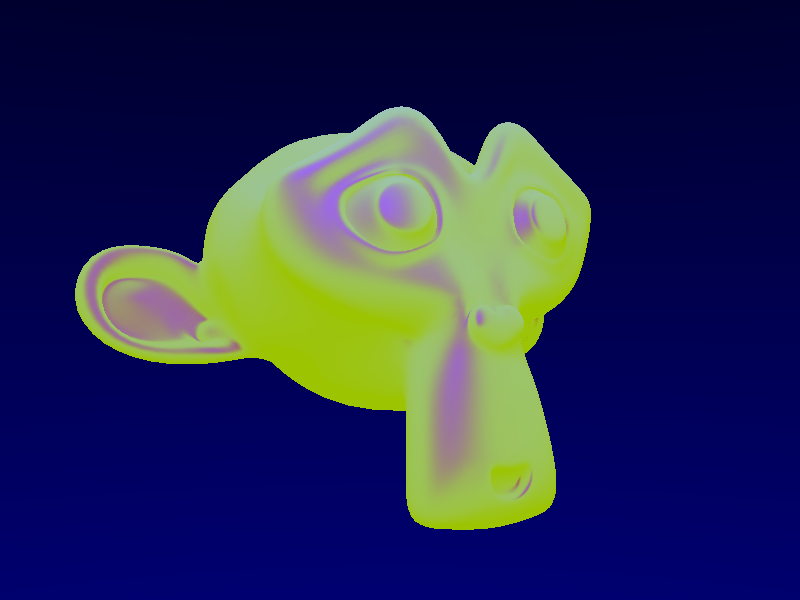
\includegraphics[width=0.25\textwidth]{images/render-hsv} }
				\subfloat[Vecteur normal de la surface]{ \label{fig:render-normal} 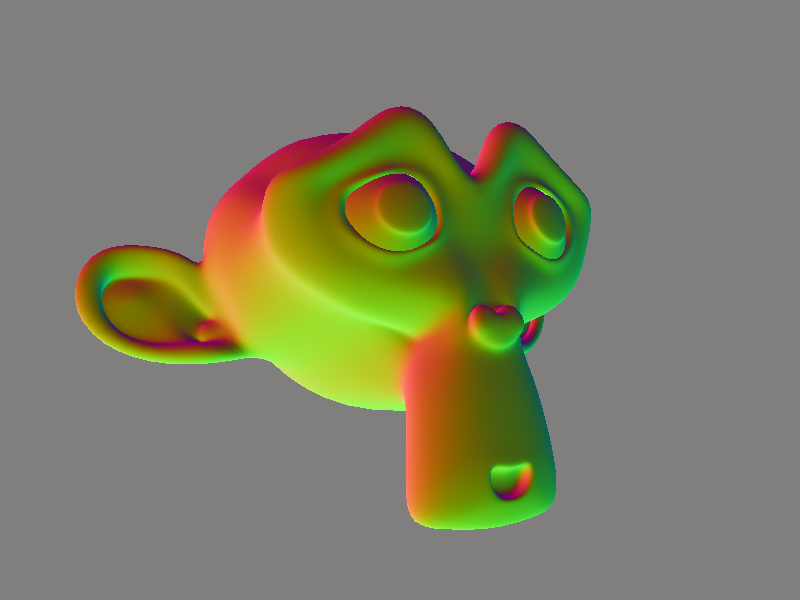
\includegraphics [width=0.25\textwidth]{images/render-normal} }
				\subfloat[Distance à l'observateur]{ \label{fig:render-depth} 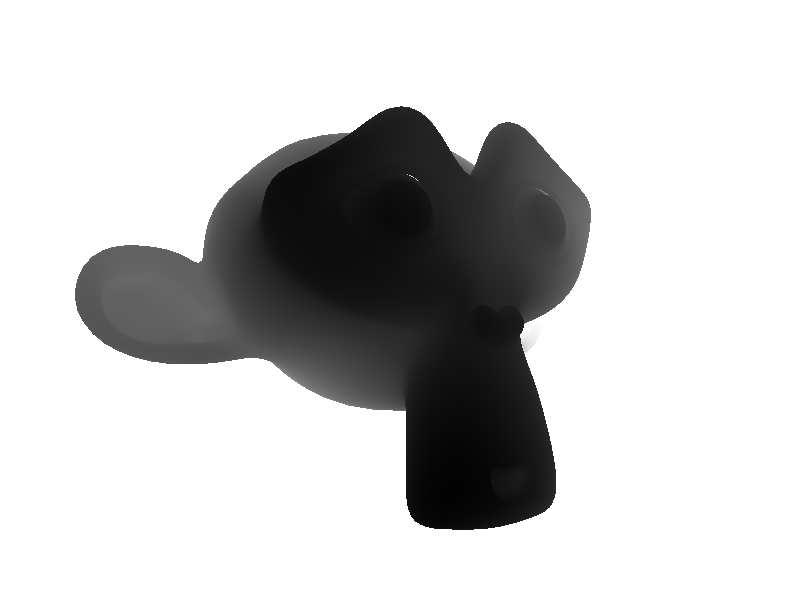
\includegraphics [width=0.25\textwidth]{images/render-depth} }
				\caption{Exemples d'espaces colorimétriques et de méta-données}
				\label{fig:color}
			\end{figure}

		\subsection{Undo / Redo}
			Un framework a souvent des mécanismes internes permettant une gestion efficace d'annulation et de répétition des opérations.
		\subsection{Édition non destructive}
			L'édition non destructive consiste à pouvoir modifier les opérations après leur application sans perte de qualité de l'image.
		\subsection{Composition non linéaire}
			La composition non linéaire permet à une opération d'utiliser le résultat d'une opération autre que celle appliquée précédemment. Idéalement
			le résultat de cette opération ne doit pas être recalculé. Cette fonctionnalité permet de combiner des effets simples afin d'obtenir des
			effets beaucoup plus complexes que ce qui est possible par composition linéaire, et permet souvent à l'utilisateur d'éviter de devoir 
			programmer ses propres effets. De nombreux logiciels présentent ainsi une interface nodale 
			comme alternative à la programmation de pixel-shaders.

		\subsection{Édition par pixel}
			Certains frameworks permettent d'éditer individuellement chaque pixel de l'image. 
		\subsection{Indépendance à la résolution}
			La description de l'image est indépendante de la résolution utilisée pour la rasterisation; Il n'y a pas de dégradation
			de la qualité de l'image quelque soit la résolution utilisée pour le rendu. L'édition par pixel et l'indépendance à la résolution
			sont deux fonctionnalités mutuellement exclusives.
		\subsection{Images gigapixels}
			Les images gigapixels sont les images constituées de plus d'un milliard de pixel, qui peuvent être plus grandes que la mémoire
			vive disponible. Il ne faut pas confondre édition d'images gigapixel et indépendance à la résolution.
			Si l'indépendance à la résolution permet de décrire des documents de tailles aussi grande
			que désirée et de les rasteriser en des images gigapixel, elle ne permet pas de décrire ou d'éditer des images
			de plus d'un milliard de pixels indépendants. 

		\subsection{Traitement d'images multiples}
			Le traitement d'images multiples consiste à savoir appliquer facilement les mêmes opérations sur un large nombre d'images similaires, 
			comme par exemple les photos d'une séance de shooting, les frames d'une vidéo ou d'un moteur 3D.

	\section{Frameworks Bitmaps}
		\subsection{Schéma de représentation de l'image}
			\begin{figure}[h]
				\centering
				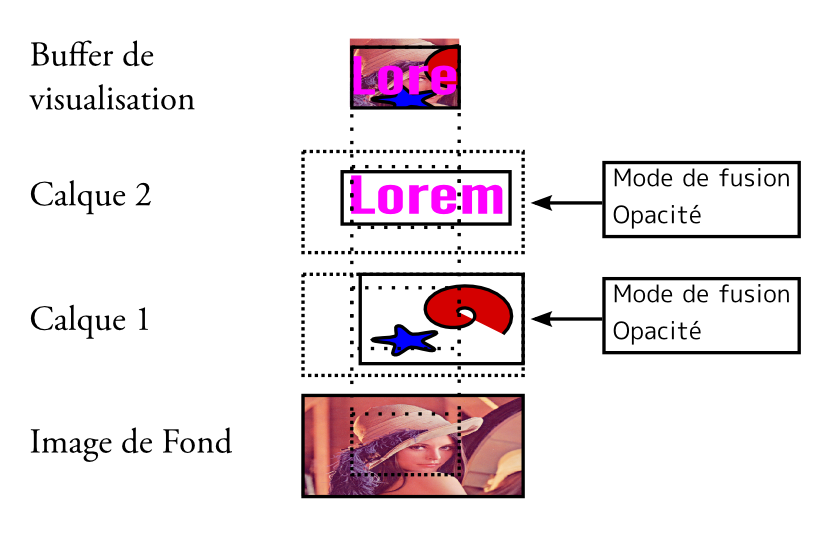
\includegraphics[width=0.6\textwidth]{images/calques}
				\caption{Représentation d'une image par calques}
				\label{fig:editbitmap}
			\end{figure}
			Dans un framework bitmap l'image est représentée directement sous sa forme rasterisée. 
			
			Une extension populaire est de décomposer l'image en une image de fond et une superposition de calques qui sont des bitmaps possédant chacun leur propre
			dimension, position, un mode de fusion, et des paramètres d'opacité. Cette extension permet à l'utilisateur de pouvoir facilement modifier des zones
			spécifiques de l'image.

			Des frameworks étendent encore ce principe en décomposant les calques en sous calques, et ce de manière récursive\footnote{Un exemple de logiciel proposant cette fonctionalité est \emph{Adobe Photoshop}}. 

		\subsection{Algorithme de rasterisation}
			Dans un framework bitmap, chaque opération est directement rasterisée à la résolution native lors de son application. 
			
			Pour visualiser une région à une échelle différente de la résolution native, On utilise un buffer de visualisation de la taille
			de cette région dans lequel la région d'intérêt est mis à l'échelle voulue après chaque rasterisation.
			
			Lorsqu'un système de calques est utilisé, on rasterise d'abord directement l'opération sur le calque modifié. On place ensuite l'image
			de fond dans le buffer de visualisation. Chaque calque y est ensuite fusionné.			
			
			Comme la plupart des opérations ne modifie qu'une petite partie de l'image, on aimerait éviter de devoir fusionner l'intégralité
			des calques à chaque fois. Il y a deux approches pour cela: La première est de demander à chaque opération de spécifier la région
			qu'elle modifie. On ne modifie ensuite le buffer de visualisation que pour cette région. 

			La deuxième approche consiste à diviser l'image de fond et les calques en une grille de sous régions aux dimensions régulières appelées
			tiles. Lors de l'application de l'opération, celle ci ne modifiera que certains tiles. Seuls les tiles correspondants dans les calques
			et l'image de fond seront fusionnés dans le buffer de visualisation. Les tiles peuvent également être traités en parallèle sur une 
			machine multiprocesseur.

			Les tiles ont d'autres intérêts que d'accélérer la rasterisation; En omettant les tiles des zones transparentes des calques ou réduit 
			l'espace mémoire qu'ils consomment. En outre, les tiles peuvent être migrés vers le disque dur lorsqu'il n'est plus possible de tous
			les stocker en mémoire, ils sont ensuite récupérés lorsqu'ils sont utilisés. 
			
			Il n'est cependant pas toujours possible d'implémenter une opération pour qu'elle fonctionne tile par tile. Dans ces cas on devra placer
			les tiles dans un buffer temporaire et les récupérer après l'opération. 

		\subsection{Fonctionnalités adaptées aux frameworks bitmaps}
			\subsubsection{Opérations de dessin}
				Étant donné qu'il n'est pas nécessaire de maintenir une liste de toutes les opérations appliquées sur l'image, les frameworks
				bitmaps sont particulièrement efficaces lorsqu'un très grand nombre de celles-ci sont utilisés ce qui est le cas pour les
				logiciels de peinture. 
			\subsubsection{Undo / Redo}
				L'undo/redo est implémenté en gardant une copie de la région/tiles modifiée par l'opération avant sa modification. 
				Il suffit ensuite de réutiliser ces copies pour obtenir la version sauvegardée. Garder les copies consomme beaucoup de mémoire,
				et une limite d'historique est nécessaire pour pallier à ce problème. En revanche, annuler ou refaire une opération ne demande
				pas de recalculer l'opération et est donc très rapide.
		\subsection{Fonctionnalités inadaptées aux frameworks bitmaps}
			\subsubsection{Modèles colorimétriques et méta-données}
				L'architecture des frameworks bitmaps limite sévèrement les possibilité de gestion de modèles colorimétriques et de méta-données.
				En effet, comme chaque opération est rasterisée dans le calque dès son application, les opérations doivent nécessairement 
				avoir le même modèle colorimétrique en entrée et en sortie. Elles doivent aussi comprendre le modèle colorimétrique et extensions du 
				calque, ce qui nécessite de devoir soit modifier les opérations à chaque ajout de nouveau type de modèles colorimétriques et d'extensions
				soit de passer par de coûteuses transformations de modèles.

				Il existe une solution permettant d'améliorer la situation : Au lieu de placer tous les composants du pixel dans un même calque, on
				divise le calque en sous calques appelés canaux qui contiennent chacun un seul composant du pixel. Les opérations sont ensuite 
				codées pour prendre des canaux en entrée et en sortie. Il est maintenant possible d'ignorer les canaux inutiles, d'avoir des canaux
				de différentes précision, et de changer la signification d'un canal lors de l'application d'une opération. 

				Cette approche à pour inconvénient de ralentir nettement les opérations, puisqu'il faut désormais accéder des zones de 
				mémoire fort éloignées pour lire ou modifier un seul pixel. 

				En pratique les framework bitmap implémentent un nombre limité de modèles colorimétriques, et imposent
				le même modèle pour tous les calques d'une image\footnote{\emph{Gimp} est passé d'un framework bitmap à un framework nodal pour
				résoudre ce problème}
			\subsubsection{Images gigapixel}
				Il est théoriquement possible de gérer des images de taille plus grande que la mémoire disponible en utilisant les tiles à
				bon escient. Mais en pratique, chaque opération nécessite d'être appliquée intégralement sur l'image à résolution native, 
				ce qui est infaisable de manière interactive pour des opérations modifiant de grandes parties de l'image.
			\subsubsection{Édition non destructive}
				L'édition non destructive requiert de garder une liste de toutes les opérations effectuées sur l'image, afin de pouvoir
				modifier l'opération désirée, et de refaire celles qui doivent être ré-appliquées. 

				Il est cependant possible d'implémenter des opérations non destructives en tant que calques à part entière. 
				Si l'opération est un filtre spatial, il faudra pouvoir étendre le buffer de rasterisation pour que le filtre ait accès aux données
				nécessaires. Et s'il s'agit d'un filtre de transformation, la zone à modifier dans le buffer de visualisation devra elle aussi
				être modifiée au fur et à mesure des filtres. Tout cela étant fort compliqué à implémenter, sans garantie de performances, 
				les frameworks confinent généralement l'édition non destructive aux filtres colorimétriques et dessin de primitives
				\footnote{\emph{Adobe Photoshop} propose des filtres non destructifs fort avancés. \emph{Gimp} est passé d'un framework
				bitmap à un framework nodal pour faciliter l'édition non destructive}.
		\subsection{Framework bitmaps, l'état de l'art}
			\begin{description}
				\item[Adobe Photoshop] Logiciel de peinture et retouche photo
				\item[Corel Painter] Logiciel de peinture
				\item[Artrage] Logiciel de peinture
				\item[Gimp $\leq$ 2.6] Logiciel de peinture et retouche photo open source
				\item[Krita] Logiciel de peinture et retouche photo open source
				\item[Blender3d] Utilisé pour la peinture de texture, Logiciel d'animation 3D.
				\item[psd] Format d'image de Photoshop
				\item[xcf] Format d'image de Gimp.
			\end{description}

	\section{Frameworks Nodaux}
		\subsection{Schéma de représentation de l'image}
			\begin{figure}[h]
				\centering
				\subfloat[En rouge les noeuds d'entrée, en orange les noeuds d'opération, en vert les noeuds de visualisation]{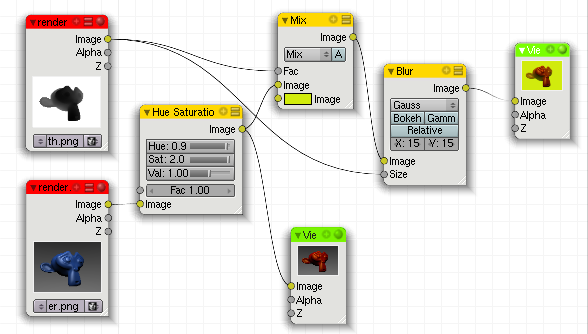
\includegraphics[width=0.8\textwidth]{images/nodes} }
				\\
				\subfloat[Image calculée par le graphe (a)]{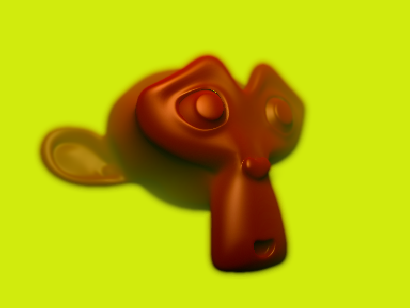
\includegraphics[width=0.4\textwidth]{images/nodes-out} }
				\caption{Exemple d'édition nodale d'images telle qu'implémenté par \emph{Blender 2.49}}
				\label{fig:editnodal}
			\end{figure}
			Les frameworks nodaux représentent l'image par un graphe composé de trois types de noeuds.
			\begin{itemize}
				\item Les noeuds d'entrée servent à spécifier les images à modifier et ne proposent que des sorties --- en rouge sur la figure~\ref{fig:editnodal}(a)
				\item Les noeuds d'opération --- en orange sur la figure~\ref{fig:editnodal}(a) --- prennent en entrée des images et/ou des canaux et/ou des paramètres,
				et proposent en sortie le résultat des images et/ou des canaux et/ou des valeurs, résultats de
				l'opération sur les entrées.
				\item Les noeuds de visualisation --- en vert sur la figure~\ref{fig:editnodal}(a) --- n'ont qu'une entrée et servent à visualiser sa valeur, que ce soit un paramètre,
				un canal ou une image. Dans le cas de canaux ou d'images, le noeud peut également spécifier une sous région
				de l'image et une échelle.
			\end{itemize}
			Le graphe est acyclique et dirigé; chaque arrête va de la sortie d'un noeud à une entrée d'un autre. Il peut
			y avoir plusieurs arrêtes partant d'une sortie, mais une seule arrivant à chaque entrée. 
		
		\subsection{Algorithme de rasterisation}
			Pour obtenir la sortie d'un noeud, il faut premièrement obtenir toutes ses entrées, et appliquer l'opération du
			noeud s'il y en a une. On appliquera donc ce principe de manière récursive en partant d'un noeud de visualisation,
			la récursion s'arrêtant au noeuds d'entrée.

			Si le noeud de visualisation spécifie une sous-région de l'image, l'algorithme fonctionne de manière identique, à
			ceci près que les opérations pouvant transformer géométriquement l'image, la région en entrée ne sera pas la même que
			la sortie. Il faut donc que le noeud soit capable d'inverser la transformation qu'il effectue afin de demander la bonne
			région à ses parents\footnote{Ce mécanisme est utilisé par le framework \emph{GEGL}.}. 

			Si le noeud de visualisation spécifie une échelle, les images fournies par les noeuds d'entrée sont mises à l'échelle avant
			leur sortie, de même que les paramètres métriques des opérations. 

			Comme une sortie peut être connectée à plusieurs entrées, une même opération peut être calculée plusieurs fois. Pour éviter
			cela, chaque noeud peut disposer d'une cache dans laquelle il place le résultat de ses sorties. 

			Les images utilisées peuvent également utiliser une représentation par tiles afin de bénéficier des avantages de gestion d'images
			volumineuses.

		\subsection{Fonctionnalités adaptées aux frameworks nodaux}
			\subsubsection{Édition non destructive}
				C'est un des gros points forts des frameworks nodaux. On peut facilement modifier les paramètres et la topologie du graphe
				et visualiser le résultat.
			\subsubsection{Composition non linéaire}
				La composition non linéaire découle de l'architecture en graphe des frameworks nodaux. Les frameworks nodaux sont d'ailleurs
				les seuls frameworks permettant une réelle édition non linéaire. 
			\subsubsection{Modèle colorimétrique}
				Un framework nodal offre une liberté totale à l'utilisateur en ce qui concerne les modèles colorimétriques. Si un noeud sort
				une image en RGB, et qu'une opération attend du YUV, il peut les connecter ensemble. Le canal R sera interprété comme Y, le G comme
				U et le B comme V\footnote{Ce mécanisme est implémenté dans \emph{Blender3d}}. S'il désire garder l'interprétation colorimétrique du RGB, il devra utiliser un noeud qui convertit le RGB en YUV.

				Intégrer un nouveau modèle colorimétrique se limite donc à créer des noeuds de conversions et les noeuds d'opération qui peuvent
				tirer bénéfice de ce nouveau modèle.

				L'édition nodale est cependant incapable de gérer les tons directs.
			
				
			\subsubsection{Images gigapixel}
				La complexité en temps et en mémoire de la rasterisation d'une image ne dépend tout au long du graphe que de la taille de
				la région du noeud de visualisation. Une borne supérieure de la taille de ces région est la résolution des écrans qui ne
				dépasse pas les quelques mégapixels. Il reste l'opération d'échelle à effectuer au niveau des région d'entrée. Si on
				dispose de mipmaps de ces images, alors il est possible d'effectuer des opérations sur images gigapixels de manière efficace
				\footnote{\emph{GEGL} implémente ce mécanisme}.
			\subsubsection{Traitement d'images multiples}
				Le même graphe peut très facilement s'appliquer sur un grand nombre d'images de manière automatique, ce qui rend ces frameworks
				particulièrement adaptés au traitement vidéo.
				
		\subsection{Fonctionnalités inadaptées aux frameworks nodaux}
			\subsubsection{Undo/Redo}
				On peut s'attendre d'un framework permettant l'édition non destructive d'exceller dans l'undo/redo. Cependant, il n'est pas
				facile de gérer les changements de paramètres des noeuds et de la topologie du graphe tout en maintenant des caches cohérentes.
				C'est pourquoi les graphes nécessitent souvent d'être rasterisés à nouveau ce qui peut prendre du temps lorsque celui ci contient
				des filtres complexes. 
			\subsubsection{Opération de dessin de primitives}
				Il est tout à fait possible de créer des noeuds dessinant des primitives, et de les connecter entre eux pour avoir une topologie
				semblant correspondre aux frameworks bitmaps ou vectoriels. 

				Un premier problème est que les frameworks nodaux appliquent les opérations de transformations sur les pixels constituant la primitive et non sur les paramètres la définissant.
				Par exemple, il sera impossible de récupérer l'apparence exacte de la primitive après une transformation d'échelle 
				la réduisant à un seul pixel. Cet exemple extrême démontre comment à chaque transformation successive, la primitive est peu à peu
				dégradée. Un framework vectoriel n'a pas ce genre de problèmes.
				
				Ensuite, un framework nodal est une entité complexe, et il devient impossible à l'utilisateur de gérer un graphe contenant 
				autant de noeuds que nécessiterait la réalisation d'une peinture. Sans parler de la consommation en mémoire du graphe, 
				et de la surcharge de calcul qu'entraîne le parcours de celui-ci.

				On ne peut pas non plus se permettre de devoir recalculer toutes les opérations de dessin à chaque Undo/Redo, à chaque édition
				non destructive et à chaque nouvelle visualisation.

				Les frameworks nodaux font donc souvent le choix d'ignorer totalement les opérations de dessin. Celles-ci sont alors effectuées
				sur les images avant leur entrée dans le graphe, et doivent être gérées par un autre framework tel qu'un framework vectoriel ou bitmap.

				Certains frameworks nodaux (GEGL) choisissent de proposer des noeuds qui regroupent une séquence d'opération de dessin en une seule.
				Ces noeuds sont donc obligés de gérer par des mécanismes interne l'undo/redo. De tels noeuds fonctionnant comme des frameworks bitmaps
				ils ne peuvent pas gérer des opérations de dessin de trop grande taille. 
				
				Ces frameworks permettent donc de peindre sur des images gigapixel, mais chaque trait de peinture doit rester de taille mégapixel,
				ce qui limite l'utilité de cette fonctionnalité dans le cadre d'édition d'images gigapixel.


			\subsubsection{Édition par pixel}
				L'édition par pixel est problématique pour les mêmes raisons qui rendent problématique le dessin de primitives.
		\subsection{Framework nodaux, l'état de l'art}
			\begin{description}
				\item[The Foundry Nuke]Logiciel de composition et post processing vidéo
				\item[Blender3D]Utilisé pour la composition et le post processing vidéo, logiciel d'animation 3D open source.
				\item[GEGL]Framework nodal open source utilisé par Gimp $\geq$ 2.7 et le logiciel d'acquisition numérique Gnome Scan.
				\item[OpenRaster]Format d'image public permettant de sauvegarder des graphes d'opérations et compatible avec GEGL.
			\end{description}

	\section{Framework vectoriel}
		\subsection{Schéma de représentation de l'image}
			\begin{figure}[h]
				\centering
				\subfloat[l'image]{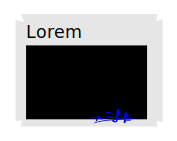
\includegraphics[width=0.33\textwidth]{images/scenegraph-img} }
				\subfloat[Le graphe de scène]{ 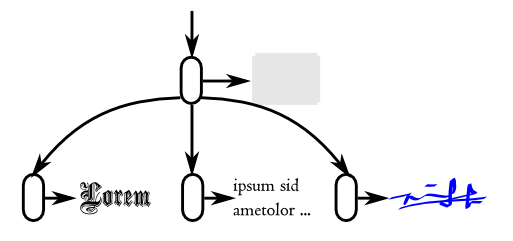
\includegraphics[width=0.66\textwidth]{images/scenegraph-graph} }
				\caption{Représentation d'une image par graphe de scène}
				\label{fig:scenegraph}
			\end{figure}
			L'image est décrite par un ensemble de primitives géométriques. Ces primitives sont organisées dans un graphe de scène. Dans un 
			graphe de scène, chaque noeud représente une transformation géométrique et une primitive. La transformation géométrique détermine
			la position, l'échelle, et la rotation de la primitive et de ses enfants. La primitive est elle décrite par son type et les paramètres
			qui déterminent sa forme et son apparence.

			Le graphe de scène est acyclique. chaque noeud peut avoir plusieurs enfants et sauf exception un seul parent. 

			L'ordre des enfants d'un noeud est important puisqu'ils déterminent l'ordre dans lequel ils seront dessinés. Ainsi les derniers
			enfants d'un noeuds seront dessinés au dessus des premiers. 

			Chaque framework a sa propre liste de primitives géométriques, mais tous disposent au moins de points, lignes, polygones, ellipses,
			texte, et courbes de bézier.

		\subsection{Algorithme de rasterisation}
			L'utilisateur commence d'abord par choisir la région qu'il veut rasteriser et à quelle résolution. Le framework crée ensuite un bitmap
			de cette taille et résolution de la couleur de fond de l'image.

			Pour dessiner un noeud du graphe, on applique sa transformation aux paramètres de sa primitive. On dessine ensuite cette 
			primitive sur le bitmap. On Dessine ensuite chaque noeud enfant dans l'ordre en leur appliquant la transformation de ce noeud.

			Cette opération est effectuée de manière récursive en partant du noeud racine de l'image.

			Afin d'éviter de dessiner les primitives qui se trouvent en dehors de la région à rasteriser, on associe à chaque noeud une boite
			qui englobe sa primitive ainsi que celles de tous ses enfants. Si la boite est en dehors de la région, on peut ignorer ce noeud et
			leurs enfants. 

			Afin d'exploiter l'accélération matérielle, la plupart des frameworks ne dessinent pas directement les primitives, mais les 
			convertissent en triangles qui sont ensuite dessinés à l'aide du matériel. Cette approche peut également s'avérer bénéfique 
			sans accélération matérielle car le dessin de triangle est souvent beaucoup plus rapide qu'un dessin analytique de la primitive,
			de plus les détails trop petits pour être vus peuvent être détectés lors de la transformation de la primitive en triangles.

		\subsection{Fonctionnalités adaptées aux frameworks vectoriels}
			\subsubsection{Édition non destructive}
				La description de la scène étant gardée en mémoire, il est facile de la modifier et d'obtenir ensuite une nouvelle visualisation.
				L'algorithme de rasterisation ne disposant généralement pas de cache\footnote{La librairie \emph{libart} est une exception notable. Il est également probable que certains frameworks fermés disposent égalemnt de systêmes de caches.}
			
				modification de l'image. Cela n'est pas un problème tant que la taille du graphe de scène reste raisonnable.
			\subsubsection{Undo / Redo}
				L'undo/redo est simple à implémenter et aussi efficace que l'édition non destructive. 
			\subsubsection{Opérations de dessin de primitives}
				Les frameworks vectoriels sont très pratiques pour éditer un dessin constitué de primitives géométriques. Cependant, la région de
				visualisation doit être rasterisée à chaque changement d'échelle ou à chaque déplacement de celle-ci. Si le nombre de primitives
				constituant le dessin est trop grand, cela ne peut plus se faire de manière interactive.
				
				Les frameworks vectoriels sont donc généralement utilisés pour les documents textuels, les cartes, les graphes, ou les dessins abstraits
				qui peuvent être décrits par un petit nombre de primitives complexes. A contrario, les images peintes utilisent 
				un trop grand nombre de primitives pour que de tels frameworks soient efficaces. 
		\subsection{Fonctionnalités inadaptées aux frameworks vectoriels}
			\subsubsection{Filtres}
				En associant les filtres aux noeuds on s'attend à ce que le filtre ne s'applique
				qu'à ce noeud et à ses enfants. Ceci nécessite de faire une rasterisation de ces noeuds dans un buffer séparé afin d'y appliquer le
				filtre, puis de réintégrer ce buffer dans le buffer en cours. Et ce de manière récursive selon qu'il y ait des filtres dans les
				noeuds enfants. 
				Tout cela ralentit nettement la rasterisation, d'autant que le rendu dans de multiples buffer ne fait pas bon ménage avec 
				l'accélération matérielle. Les frameworks proposent parfois de tels filtres, mais les performances suivent rarement.
				
				Le format vectoriel SVG propose des sémantiques de filtres plus complexes. Le fait qu'aucun framework ne les implémente correctement
				atteste de la difficulté de cette entreprise. 
			\subsubsection{Composition non linéaire}
				La structure arborescente du scene graphe ne permet pas de décrire des compositions non linéaires.
			\subsubsection{Édition par pixel}
				Éditer un pixel requiert de créer une primitive couvrant uniquement ce pixel. Si cela est possible, cela crée rapidement une trop
				grande quantité de noeuds au fur et a mesure que chaque pixel est modifié. De plus, une telle description pose de gros problèmes
				d'anti-aliasing pour les résolutions non natives\footnote{Ce problème est détaillé au chapitre \emph{Anti-aliasing}.} 
			\subsubsection{Images gigapixel}
				Les frameworks vectoriels décrivant l'image de manière analytique peuvent gérer des images de toutes tailles et résolutions. De 
				plus la description vectorielle utilise beaucoup moins de mémoire. Ces frameworks sont donc pour l'instant la solution de choix
				pour décrire des documents de grande taille. Cependant il ne s'agit pas là à proprement parler d'images gigapixel.  
			\subsubsection{Modèles colorimétriques}
				Tant la description de l'image que l'algorithme de rasterisation sont peu adaptés au support de multiples modèles 
				colorimétriques, à une exception près, le modèle par nuancier. Dans ce cas chaque primitive est associée à une couleur du nuancier,
				et à une opacité. L'image peut ainsi être envoyée sous forme vectorielle à l'imprimante qui va imprimer les primitives une à une
				en respectant la structure du graphe de scène. L'image peut également être rasterisée pour obtenir pour chaque pixel la proportion
				des encres à utiliser. 
		\subsection{Framework Vectoriels, l'état de l'art}
			\begin{description}
				\item[Adobe Illustrator]Logiciel d'édition graphique vectorielle. 
				\item[Corel Draw]Logiciel d'édition graphique vectorielle.
				\item[Adobe Flash]Logiciel d'animation 2D
				\item[Inkscape]Logiciel open source d'édition graphique vectorielle.
				\item[libart]Librairie open source de rendu et d'édition graphique vectorielle, utilisée par Gnome Canvas, Inkscape.
				\item[Cairo]Librairie open source de rendu et d'édition graphique vectorielle, utilisée par Mozilla Firefox, Webkit, Moonlight,
				FontForge, Poppler, Gtk+
				\item[ai]Format d'image vectorielles.
				\item[SVG]Format public d'images vectorielles.
				\item[ps]Format et langage de programmation public décrivant des images vectorielles, obsolète à de nombreux égards mais toujours utilisé pour l'impression de documents.  
			\end{description}

	\section{Mégatexturing ou Sparse Virtual Textures}
		Les scènes 3D interactives sont de plus en plus grandes et détaillées. Or les détails sont limités par la taille des textures que l'on peut y
		appliqué, qui sont elle même limitées par l'espace mémoire disponible sur la carte graphique. On était donc condamné jusqu'il y a peu à utiliser
		une des trois techniques suivantes, ou de les combiner : 
		\begin{itemize}
			\item Une grande texture basse résolution
			\item Une petite texture haute résolution qui se répète sur les surfaces
			\item Des textures vectorielles.
		\end{itemize}
		Aucune de ces techniques ne peuvent texturer un large environnement de manière convaincante. 

		Le Mégatexturing, appelé aussi Sparse Virtual Texture est donc une technique d'affichage de textures plus qu'un framework à part entière. Le but de 
		cette technique est de permettre l'affichage et l'édition d'images gigapixel en tant que textures de scènes 3D interactives. Une image gigapixel
		étant suffisamment grande  pour couvrir l'intégralité de l'environnement à haute résolution.

		\subsection{Schéma de représentation de l'image}
			\begin{figure}[h]
				\centering
				\subfloat[La pyramide de tile représentant l'image complète]{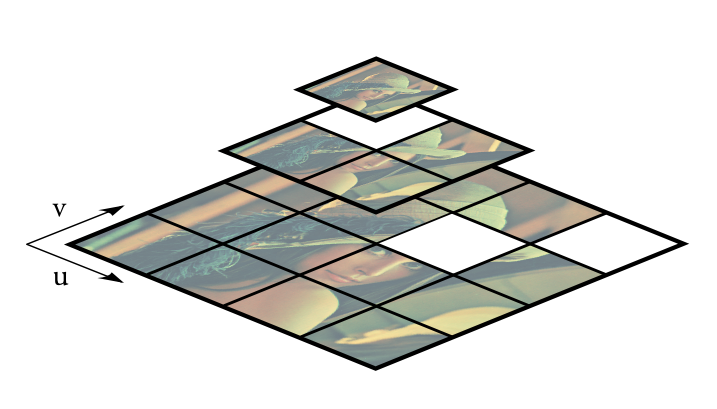
\includegraphics[width=0.6\textwidth]{images/megatextures-pyramid} }
				\subfloat[La texture virtuelle, composée de tiles de la pyramide]{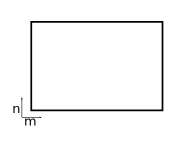
\includegraphics[width=0.4\textwidth]{images/megatextures-virtual} }
				\caption{Mégatexture}
				\label{fig:editmegatex}
			\end{figure}
		L'image est représentée par deux structures différentes, l'une se trouvant sur le disque et l'autre en mémoire.
		Celle qui se trouve sur le disque est la plus volumineuse des deux. Elle est composée d'une pyramide creuse de tiles. 

		Cette structure consiste en l'image gigapixel complète, divisée en tiles, les régions vides ou facultatives de l'image étant représentées par une absence
		de tiles, afin d'économiser de la mémoire. La structure contient aussi tous les mipmaps de cette image sous forme de tiles de dimensions identiques.

		En mémoire se trouve une texture, appelée \emph{texture virtuelle} qui a la taille maximum supportée par le matériel d'accélération, 
		ce qui est beaucoup moins que l'image originale. Cette texture est composée de tiles se trouvant dans la pyramide.
		
		\subsubsection{Affichage de l'image}
			Pour afficher une texture sur un maillage 3D, on assigne à chaque vertice  du maillage une coordonnée $u,v$ correspondant à un pixel de cette texture.
			de la texture. Comme nous désirons afficher la texture gigapixel, ces coordonnées correspondent aux pixels de cette texture.
			Celle-ci est cependant trop grande pour pouvoir être utilisée telle quelle.
			
			Pour résoudre ce problème on place les tiles qui nous intéressent dans une texture virtuelle qui est suffisamment petite pour pouvoir
			être utilisée pour l'affichage. Un \emph{pixel shader} est ensuite utilisé pour traduire lors de l'affichage les coordonnées $u,v$ de la
			texture gigapixel en les coordonnées $m,n$ de la texture virtuelle. 

			Pour déterminer quels tiles nous intéressent, on s'aide d'un premier rendu dans lequel on examine quelles régions de la texture gigapixel
			sont affichées, et à quelle résolution. On sélectionne ensuite les tiles qui couvrent cette zone avec la résolution la plus proche de celle
			affichée. Comme la résolution de l'écran est plus petite que celle de la taille de la texture virtuelle, on disposera toujours d'une place
			suffisante pour couvrir la quantité de texture affichée.

			Récupérer les tiles sur le disque implique un délai non négligeable. Le megatexturing incorpore des techniques permettant de pallier à
			ce problème qui sortent du cadre de cette présentation.

		\subsubsection{Édition de l'image}
			Pour générer et éditer l'image gigapixel, on utilise la technique précédente pour l'affichage, et on utilise les techniques de framework 
			bitmap pour appliquer les opérations; Celles-ci sont directement rasterisées dans la pyramide de tiles.
		\subsubsection{État de l'art du Mégatexturing}
			Le Mégatexturing à été popularisé par id Software pour son utilisation dans le moteur de jeu idTech4 et idTech5\cite{megatex1}\cite{megatex2}. Cette technique est utilisé
			par les jeux utilisant ces moteurs. D'autres moteurs tels que Torque ont réimplémenté cette technique.

	\section{Comparaison des différents framework}

	\begin{table*}
		\begin{tabular*}{\textwidth}{@{\extracolsep{\fill}} | l || c | c | c | c |}
			\hline
			Fonctionnalité	 		& Bitmap 		& Nodal 		& Vectoriel 		& Himalaya 	\\
			\hline \hline	                                                                                                          
			Dessin de primitives	   	& $\medbullet$		& $\ominus$		& $\medbullet$	 	& $\medbullet$	\\
			Peinture		   	& $\medbullet$		& $\ocircle$		& $\ominus$		& $\medbullet$	\\
			Filtres	colorimétriques	   	& $\medbullet$		& $\medbullet$		& $\ominus$		& $\medbullet$	\\
			Filtres	spatiaux	   	& $\medbullet$		& $\medbullet$		& $\ominus$		& $\ocircle$	\\
			Transformations vectorielles   	& $\ocircle$		& $\ocircle$		& $\medbullet$	 	& $\ocircle$	\\
			Transformations bitmap   	& $\medbullet$		& $\medbullet$		& $\ominus$	 	& $\ominus$	\\
			Modes de fusion		   	& $\medbullet$		& $\medbullet$		& $\medbullet$	 	& $\medbullet$	\\
			Modèles colorimétriques	   	& $\ominus$		& $\medbullet$		& $\ominus$	 	& $\medbullet$	\\
			Ton direct		   	& $\ominus$		& $\ocircle$		& $\medbullet$	 	& $\ocircle$	\\
			Modèles étendus		   	& $\ocircle$		& $\medbullet$		& $\ocircle$	 	& $\ominus$	\\
			Undo/Redo		   	& $\medbullet$		& $\ominus$		& $\medbullet$	 	& $\medbullet$	\\
			Édition non destructive	   	& $\ocircle$		& $\medbullet$		& $\medbullet$	 	& $\medbullet$	\\
			Composition non linéaire	& $\ocircle$		& $\medbullet$		& $\ocircle$	 	& $\medbullet$	\\
			Édition par pixel		& $\medbullet$		& $\ocircle$		& $\ocircle$	 	& $\ominus$	\\
			Indépendance à la résolution	& $\ocircle$		& $\ominus$		& $\medbullet$	 	& $\ocircle$	\\
			Images Gigapixel		& $\ocircle$		& $\medbullet$		& $\medbullet$	 	& $\medbullet$	\\
			Traitement d'images multiples	& $\ominus$		& $\medbullet$		& $\ocircle$	 	& $\ominus$	\\
			\hline
			\multicolumn{5}{|l|}{ \tiny $\medbullet$ : Fonctionnalité adaptée au framework.} \\
			\multicolumn{5}{|l|}{ \tiny $\ominus$ : Fonctionnalité implémentable dans le framework, mais de manière limitée ou peu performante.} \\ 
			\multicolumn{5}{|l|}{ \tiny $\ocircle$ : Fonctionnalité inadaptée au framework.}	\\
			\hline
		\end{tabular*}
		\caption{Grille de comparaison des fonctionnalités. }
		\label{comparaison}
	\end{table*}

	Le tableau~\ref{comparaison}, (page~\pageref{comparaison}) permet d'avoir une vision globale des fonctionnalités supportées par les différents 
	types de framework. On remarque que les frameworks proposent des fonctionnalités très différentes, ce qui explique pourquoi chaque 
	domaine d'application tend à préférer un framework en particulier.

	Ce tableau permet aussi de comparer les frameworks existants aux fonctionnalités adaptées au framework Himalaya qui est présenté dans ce mémoire. Cette
	comparaison reste en partie théorique puisque toutes ces fonctionnalités n'ont pas été implémentées et soumises à des tests utilisateurs. 
	
	Néanmoins ce framework propose une combinaison intéressante de fonctionnalité en combinant Peinture, Dessin de primitives, Édition non destructive, 
	Composition non linéaire et Images gigapixel. Non repris dans ce tableau est la possibilité -- encore théorique -- de pouvoir utiliser la technique
	de mégatexture en combinaison avec \emph{Himalaya} afin de permettre l'édition non destructive des textures d'une scène 3D temps réel.

	La suite de ce mémoire se concentrera sur la présentation de l'architecture et des fonctionnalités de base du framework Himalaya, pour se concentrer
	ensuite sur l'implémentation et l'évaluation par test utilisateurs des fonctionnalités de peinture et d'édition d'images gigapixel, combinaison de
	fonctionnalité n'étant proposée par aucun des frameworks existants.

